\documentclass[12pt]{article}
\usepackage[utf8]{inputenc}
\usepackage{geometry}
\geometry{a4paper, margin=1in}
\usepackage{graphicx}
\usepackage{hyperref}
\usepackage{amsmath}
\usepackage{pgfplots}
\pgfplotsset{compat=1.18}

\title{Proyecto Integral 0001}
\author{Gerente de Proyecto: John Doe}
\date{24 de septiembre de 2024}

\begin{document}

\maketitle

\tableofcontents
\newpage

\section{Introducción}
Este memorando del proyecto integral proporciona una actualización detallada sobre el proyecto ABC, describiendo el progreso, los principales riesgos, las estrategias de mitigación y los hitos próximos. El memorando está estructurado para ofrecer información detallada sobre cada fase del proyecto y resaltar las áreas clave de enfoque para los próximos meses.

El objetivo del proyecto es aumentar el rendimiento del sistema en un 30\%, haciéndolo más eficiente y escalable para los requisitos futuros. Desde la última actualización en agosto, hemos logrado avances significativos, pero persisten desafíos, particularmente en la integración de APIs y la optimización de bases de datos.

\section{Resumen del Proyecto}
El proyecto ABC se divide en tres fases:
\begin{itemize}
    \item \textbf{Fase 1: Recopilación de Requisitos} (Completado)
    \item \textbf{Fase 2: Desarrollo} (En curso)
    \item \textbf{Fase 3: Pruebas y Despliegue} (Programado)
\end{itemize}

\subsection{Fase 1: Recopilación de Requisitos}
La Fase 1 se completó el 15 de agosto de 2024. Durante esta fase, colaboramos con los principales interesados para recopilar requisitos completos. Esto aseguró la alineación entre el equipo de desarrollo y los objetivos empresariales.

El proceso de recopilación de requisitos reveló varias áreas de mejora potencial, incluyendo la mejora de la seguridad del sistema, la ampliación de la infraestructura para soportar usuarios adicionales y la integración de APIs de terceros para aumentar la funcionalidad.

\subsection{Fase 2: Desarrollo}
La Fase 2, que comenzó a mediados de agosto, se ha dividido en dos líneas de trabajo clave: desarrollo del frontend e integración del backend.

\paragraph{Desarrollo del Frontend} La interfaz de usuario ha sido rediseñada para mejorar la experiencia del usuario. Los comentarios del equipo de diseño sugieren que la nueva interfaz reduce la fricción del usuario, particularmente en entornos de alto tráfico.

\paragraph{Integración del Backend} El sistema de backend está experimentando importantes actualizaciones, que incluyen:
\begin{itemize}
    \item Implementación de una arquitectura de microservicios.
    \item Mejora en la gestión de bases de datos.
    \item Integración de APIs.
\end{itemize}

Actualmente enfrentamos retrasos en la integración de las APIs del backend, lo que ha impactado el cronograma del proyecto. Sin embargo, estamos agregando recursos adicionales para asegurarnos de que este retraso no se extienda a la siguiente fase.

\section{Estado Actual}
Al 24 de septiembre de 2024, hemos logrado un progreso significativo tanto en el desarrollo del frontend como en la integración del backend.

\subsection{Métricas de Progreso}
La siguiente tabla proporciona una visión general del progreso del proyecto, detallando el porcentaje completado para los componentes clave de la Fase 2.

\begin{table}[h!]
\centering
\begin{tabular}{|c|c|c|}
\hline
\textbf{Componente} & \textbf{Fecha de Finalización Prevista} & \textbf{Progreso (\%)} \\
\hline
Desarrollo del Frontend & 5 de octubre de 2024 & 80\% \\
Desarrollo del Backend & 20 de octubre de 2024 & 60\% \\
Integración de APIs & 1 de octubre de 2024 & 50\% \\
Optimización de Bases de Datos & 10 de octubre de 2024 & 70\% \\
\hline
\end{tabular}
\caption{Resumen del Progreso de Componentes Clave}
\end{table}

\subsection{Gráfico de Burndown de Desarrollo}
A continuación se muestra un gráfico de burndown que refleja el progreso del equipo en las últimas seis semanas. Se rastrea el trabajo restante contra el trabajo total planificado para la Fase 2.

\begin{center}
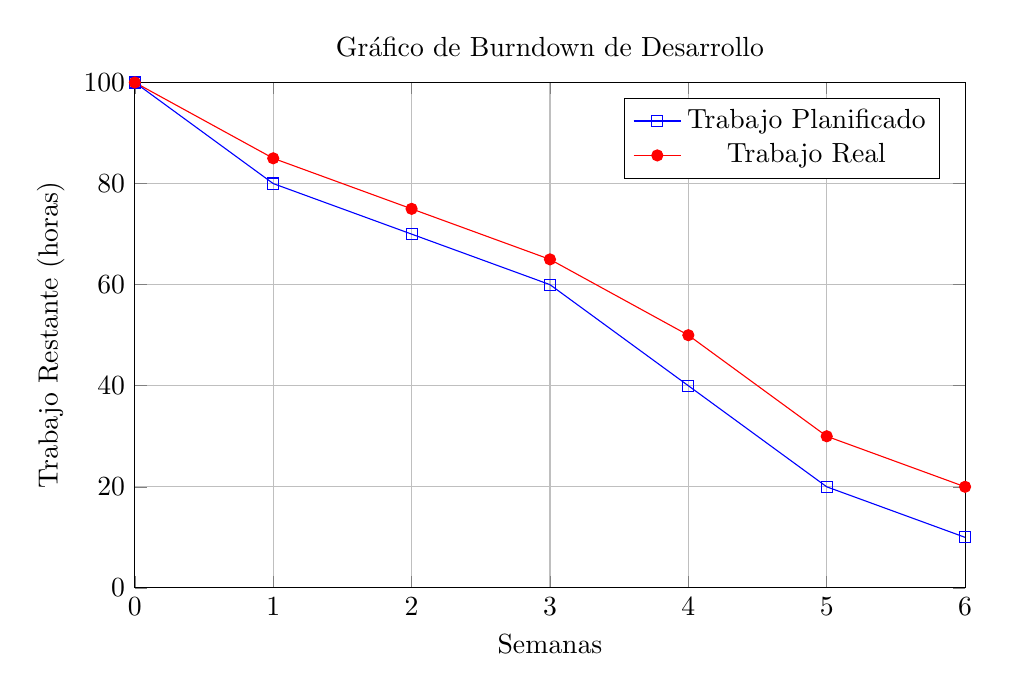
\begin{tikzpicture}
\begin{axis}[
    title={Gráfico de Burndown de Desarrollo},
    xlabel={Semanas},
    ylabel={Trabajo Restante (horas)},
    xmin=0, xmax=6,
    ymin=0, ymax=100,
    xtick={0,1,2,3,4,5,6},
    ytick={0,20,40,60,80,100},
    legend pos=north east,
    grid=major,
    width=\linewidth,
    height=8cm
]
\addplot[color=blue,mark=square] coordinates {
    (0, 100) (1, 80) (2, 70) (3, 60) (4, 40) (5, 20) (6, 10)
};
\addplot[color=red,mark=*] coordinates {
    (0, 100) (1, 85) (2, 75) (3, 65) (4, 50) (5, 30) (6, 20)
};
\legend{Trabajo Planificado, Trabajo Real}
\end{axis}
\end{tikzpicture}
\end{center}

\newpage
\section{Principales Riesgos y Estrategias de Mitigación}
Se han identificado varios riesgos, con las correspondientes estrategias de mitigación que se detallan a continuación:

\subsection{Riesgo 1: Retrasos en la Integración de APIs}
\textbf{Descripción:} Los retrasos en la integración de APIs de terceros han causado un cuello de botella en el desarrollo del backend. Esto podría retrasar la finalización del backend en dos semanas.

\textbf{Estrategia de Mitigación:} Se ha asignado un desarrollador adicional al equipo de integración de APIs para acelerar el proceso. También estamos en conversaciones con el proveedor externo para agilizar los cambios necesarios.

\subsection{Riesgo 2: Problemas de Escalabilidad de la Base de Datos}
\textbf{Descripción:} Las primeras pruebas han revelado posibles problemas en la escalabilidad de la base de datos. Esto podría ocasionar cuellos de botella de rendimiento cuando el sistema esté bajo carga pesada.

\textbf{Estrategia de Mitigación:} El equipo de arquitectura está revisando el diseño de la base de datos. Planeamos implementar una solución de escalado horizontal que distribuirá la carga entre varias instancias de base de datos.

\section{Próximos Hitos}
Los siguientes pasos del proyecto incluyen los siguientes hitos clave:

\begin{itemize}
    \item \textbf{1 de octubre de 2024:} Completar la integración de APIs.
    \item \textbf{10 de octubre de 2024:} Comenzar las pruebas integrales del sistema, incluyendo pruebas de rendimiento y seguridad.
    \item \textbf{20 de octubre de 2024:} Finalizar el desarrollo del backend, incluyendo la optimización de bases de datos.
    \item \textbf{5 de noviembre de 2024:} Iniciar el despliegue por fases en los entornos de staging.
    \item \textbf{15 de noviembre de 2024:} Despliegue final en producción.
\end{itemize}

\section{Conclusión}
El proyecto ABC está progresando bien, aunque persisten algunos riesgos, particularmente en la integración de APIs y la escalabilidad de la base de datos. Con los recursos adicionales asignados al proyecto y la estrecha colaboración con los proveedores externos, esperamos cumplir con los plazos revisados. Se proporcionará una actualización detallada en el próximo memorando del proyecto, programado para el 24 de octubre de 2024.

\end{document}
